% CS224W project proposal -- Autumn 2026
% Compile: pdflatex + bibtex (Overleaf: upload this folder), or `tectonic main.tex`.
% Format required by the course: NeurIPS'22 style, 2 pages without references, no abstract.
\documentclass{article}

\usepackage[final]{neurips_2022}
\makeatletter
\renewcommand{\@noticestring}{CS224W: Machine Learning with Graphs, Stanford University, Autumn 2026. Project proposal (type 1: real-world application).}
\makeatother

\usepackage{xcolor}
\definecolor{mappath}{HTML}{9E5400}
\definecolor{graphpath}{HTML}{0B6065}
\usepackage[utf8]{inputenc}
\usepackage[T1]{fontenc}
\usepackage[colorlinks=true,linkcolor=black,citecolor=graphpath,urlcolor=graphpath]{hyperref}
\usepackage{url}
\usepackage{booktabs}
\usepackage{amsfonts,amsmath}
\usepackage{microtype}
\usepackage{graphicx}
\usepackage{tikz}
\usetikzlibrary{arrows.meta,positioning,fit}


\title{Where Should a Robot Swarm See Its Neighbors?\\ Communication-Range Transfer in a GNN Coverage Policy}

\author{%
  Lo\"ic Poisson \quad Harold Gardon \quad Claire Fitussi \\
  Stanford University \\
  \texttt{\{lpoisson, gardon21, cfitussi\}@stanford.edu}
  % TODO(Loic): check that lpoisson is your SUNet ID.
}

\begin{document}
\maketitle
\vspace{-1.2em}

% =====================================================================
\section{Application domain}
% =====================================================================

\paragraph{Problem.}
In \emph{coverage control}, $N$ robots must spread over an area so that their sensors watch the regions that matter, described by an \emph{importance density field} (IDF) $\phi$ that the robots do not know in advance~\citep{cortes2004coverage}. Each robot only sees a $64\times64$\,m sensor footprint and can only exchange messages with robots within its \emph{communication range}~$R$; there is no central computer. The communication network is a graph $G_R=(V,E_R)$ with one node per robot and an edge $(i,j)$ whenever $\|p_i-p_j\|\le R$. This makes decentralized control a natural graph learning problem: every robot must decide what to send to its neighbors and how to combine what it receives~\citep{tolstaya2019flocking}.

\paragraph{Dataset.}
We use the \textbf{CoverageControl} library~\citep{coveragecontrol} (GPL-3.0, \texttt{pip install coverage\_control}), released with the LPAC paper~\citep{agarwal2025lpac}. It provides (i) a simulator of 32 robots in a $1024\times1024$\,m world, with IDFs drawn as mixtures of 32 random Gaussians; (ii) the published LPAC checkpoint and the 11 evaluation environments it ships with; and (iii) scripts that generate imitation data by running a \emph{clairvoyant} centroidal-Voronoi (CVT) controller that knows $\phi$ and all positions. One training sample is the state of all 32 robots at one time step: each robot's four $32\times32$ input maps, its position, the communication graph, and the clairvoyant's velocity as target. As in the paper, a training set has 100{,}000 samples; we also saved 40 new evaluation environments. Everything we use is public; our generated environments, data-generation configurations and code will be released in our repository\footnote{\url{https://github.com/loicpoisson/lpac-communication-range} (made public before the final submission).} before the final submission.

\paragraph{Task and metric.}
The learned policy maps each robot's local observations and messages to a velocity, i.e.\ node-level regression on $G_R$, trained by imitation (mean squared error to the clairvoyant). We evaluate it in closed loop for 600 steps and report the paper's metric: the coverage cost $J=\int\phi(q)\min_i\|q-p_i\|^2\,dq$ averaged over the episode, divided by the clairvoyant's cost on the same environment (lower is better; centralized CVT scores about 2.5). Our protocol varies the \emph{test-time} range $R\in\{128,256,512,768,1024\}$\,m, reports means over environments with paired differences, and uses three training seeds to set noise thresholds.

\paragraph{Why this dataset.}
LPAC is a recent published GNN policy whose authors report an unexplained anomaly: performance degrades when $R$ grows (their Sec.~VI-H). The simulator controls graph density exactly, the model is written in PyTorch Geometric~\citep{fey2019pyg}, and a full training run takes 2--4\,h on one free Stanford FarmShare GPU.

% =====================================================================
\section{Graph ML techniques}
% =====================================================================

\begin{figure}[t]
\centering
\begin{minipage}[c]{0.52\linewidth}
\centering
\resizebox{\linewidth}{!}{%
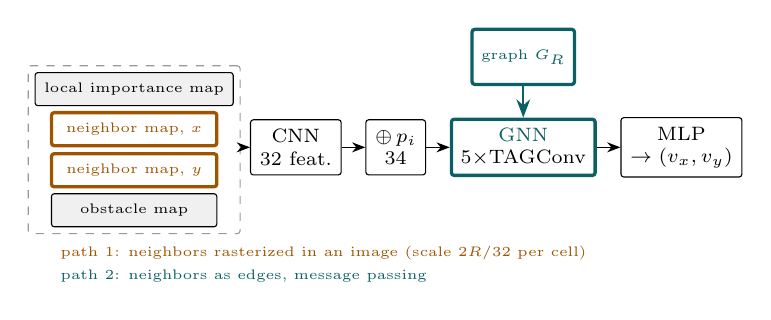
\begin{tikzpicture}[font=\scriptsize, >=Stealth,
  box/.style={draw, rounded corners=1pt, minimum height=7mm, align=center, fill=white},
  inp/.style={draw, rounded corners=1pt, minimum width=21mm, minimum height=4.2mm, align=center, font=\tiny}]
  \node[inp, fill=black!6] (loc) {local importance map};
  \node[inp, draw=mappath, very thick, below=0.6mm of loc] (mx) {\textcolor{mappath}{neighbor map, $x$}};
  \node[inp, draw=mappath, very thick, below=0.6mm of mx] (my) {\textcolor{mappath}{neighbor map, $y$}};
  \node[inp, fill=black!6, below=0.6mm of my] (obs) {obstacle map};
  \node[box, right=4mm of mx.south east, anchor=west, yshift=0mm] (cnn) {CNN\\32 feat.};
  \node[box, right=3mm of cnn] (cat) {$\oplus\,p_i$\\34};
  \node[box, draw=graphpath, very thick, right=3mm of cat] (gnn) {\textcolor{graphpath}{GNN}\\5$\times$TAGConv};
  \node[box, draw=graphpath, very thick, above=4mm of gnn, font=\tiny] (graph) {\textcolor{graphpath}{graph $G_R$}};
  \node[box, right=3mm of gnn] (mlp) {MLP\\$\to(v_x,v_y)$};
  \node[draw=black!40, dashed, rounded corners=1pt, inner sep=0.8mm, fit=(loc)(obs)] (inputs) {};
  \draw[->] (inputs.east |- cnn.west) -- (cnn.west);
  \draw[->] (cnn) -- (cat); \draw[->] (cat) -- (gnn); \draw[->] (gnn) -- (mlp);
  \draw[->, graphpath, thick] (graph) -- (gnn);
  \node[font=\tiny, text=mappath, align=left, below=1.2mm of obs.south west, anchor=north west] {path 1: neighbors rasterized in an image (scale $2R/32$ per cell)};
  \node[font=\tiny, text=graphpath, align=left, below=4.2mm of obs.south west, anchor=north west] {path 2: neighbors as edges, message passing};
\end{tikzpicture}}
\end{minipage}\hfill
\begin{minipage}[c]{0.46\linewidth}
\centering
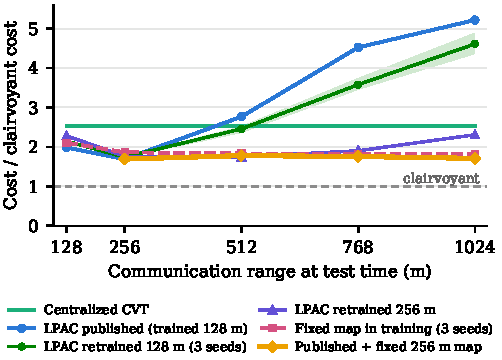
\includegraphics[width=\linewidth]{figures/results.pdf}
\end{minipage}
\caption{\textbf{Left:} LPAC on one robot. Neighbors enter twice: drawn in a $32\times32$ neighbor map read by the CNN (path 1) and as edges of $G_R$ read by the GNN (path 2). \textbf{Right:} cost (lower is better), mean over the 11 released environments. Models trained at 128\,m collapse at larger test ranges; drawing the neighbor map at a fixed 256\,m scale removes the collapse, at test time or during training on mixed ranges.}
\label{fig:main}
\end{figure}

\paragraph{Model: LPAC~\citep{agarwal2025lpac}.}
Each robot runs the same network (Fig.~\ref{fig:main}, left). A CNN encodes four $32\times32$ maps into 32 features, the robot position is appended, five TAGConv layers~\citep{du2017tagconv} with $K=3$ exchange information over $G_R$, and an MLP outputs the velocity. With node features $X$, adjacency $A$ and degree matrix $D$,
\begin{equation}
X^{(\ell+1)}=\mathrm{ReLU}\Big(\textstyle\sum_{k=0}^{K}\big(D^{-1/2}AD^{-1/2}\big)^{k}X^{(\ell)}W_k^{(\ell)}\Big),
\end{equation}
the GCN propagation~\citep{kipf2017gcn} applied up to 15 times in total. Two of the CNN's input channels form a \emph{neighbor map}: robot $j$ within range is written into cell $c_{ij}=\mathrm{round}\big((p_j-p_i)\tfrac{32}{2R}+15.5\big)$ with value $(p_j-p_i)/R$, values summed per cell. GNNs suit this problem because message passing is exactly local communication: the policy is decentralized, permutation-equivariant, and independent of team size~\citep{tolstaya2019flocking}.

\paragraph{Preliminary findings.}
(1)~\emph{Reproduction.} Retrained, LPAC matches the published model (1.74 vs 1.69 at 256\,m). Trained separately at 128, 256, 512 and 1024\,m and tested at its own range, it beats both CVT baselines at every range, as in the paper, but the drop beyond 512\,m reported there does not appear in our runs (2.15 / 1.76 / 1.79 / 1.80, one seed). (2)~\emph{Transfer collapse.} The model trained at 128\,m reaches 5.22 at 1024\,m, worse than both baselines in all 11 environments; three retrained seeds reproduce this (Fig.~\ref{fig:main}). (3)~\emph{Cause.} At 1024\,m, capping $G_R$ to 4 neighbors leaves the cost at 5.11, while drawing only the neighbor map at a fixed 256\,m scale brings it to 1.71, the 256\,m performance (paired $+0.02\pm0.16$), on every model and 40 unseen environments; TAGConv outputs keep a high effective rank, ruling out over-smoothing. (4)~\emph{Heterogeneous teams.} When a fraction of robots hears at 1024\,m and the rest at 128\,m, the cost grows convexly with that fraction, while the fixed-scale map keeps it flat (1.7--2.1).

\paragraph{Planned techniques.}
Our question is \emph{where neighbor geometry should live, and at which scale}: in a rasterized image read by a CNN, or on the edges of the graph. Under identical data and budgets we compare: (a)~inference-time interventions on each input path; (b)~training-time remedies: mixed communication ranges, a domain-randomization baseline~\citep{tobin2017domain} (1.9 at 1024\,m but 0.3 worse at 256\,m), the robot's own range as an input (no gain over mixed ranges), and a fixed-scale map used during training, our best recipe so far (three seeds: 1.86 at 256\,m, 1.81--1.83 up to 1024\,m, $+0.12\pm0.05$ behind LPAC at 256\,m); (c)~graph-native encoders that drop the map and put the relative position $p_j-p_i$, scaled by a fixed length, on the edges, as in related swarm policies~\citep{muthusamy2024generalizability,owerko2025mast}: GATv2~\citep{brody2022gatv2} underfits, and a PointNet edge layer~\citep{qi2017pointnetpp} before the TAGConv stack degrades little with range (2.01 to 2.58, three seeds) but fails when trained on mixed ranges, since its inputs grow with $R$; we will test bounded edge features (unit direction, saturating distance); (d)~heterogeneous teams, with one specialist model per range. Success: within 0.05 of LPAC at 256\,m, flat up to 1024\,m, with no test-time fix (three seeds).

\bibliographystyle{plainnat}
\small
\bibliography{refs}

\end{document}
